\chapter{Fundamentals}

\begin{figure}
	\centering
    \def\svgwidth{\textwidth}
%    \includestandalone[width=\textwidth]{figures/fig/lstmtikz}
    \input{figures/inkscape/aimldl.pdf_tex} %use full path to know the location of pdftex
    \caption{AIMLDL}
    \label{fig:ai_ml_dl}
\end{figure}
\begin{figure}
	\centering
    \def\svgwidth{\columnwidth}
%    \includestandalone[width=\textwidth]{figures/fig/lstmtikz}
    \input{figures/inkscape/jaguarsensorconstellation.pdf_tex} %use full path to know the location of pdftex
    \caption{AIMLDL}
    \label{fig:Sensors}
\end{figure}
\iffalse
\begin{figure}[h]
    \begin{center}
        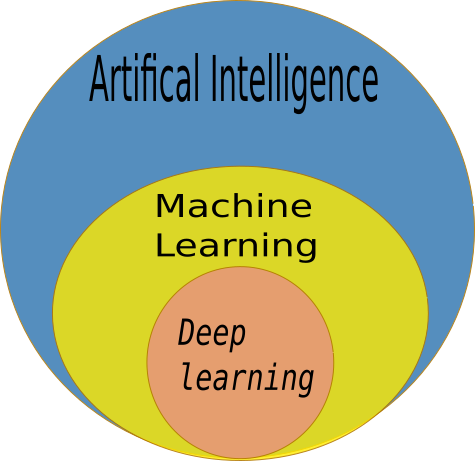
\includegraphics[width =0.3\textwidth]{figures/inkscape/aimldl.png}
    \end{center}
    \caption{Representing Artificial Intelligence, Machine Learning and Deep Learning as a
    subset of one another.}
    \label{fig:ai_ml_dl}
\end{figure}


\begin{figure}
	\centering
    \includestandalone[width=\textwidth]{figures/fig/multilayer_perceptron}
    \caption{Multilayer Perceptron.}
    \label{fig:multilayer_perceptron}
\end{figure}

\begin{figure}
	\centering
    \includestandalone[width=\textwidth]{figures/fig/SLsetup}
    \caption{Supervised Learning set up}
    \label{fig:SL_setup}
\end{figure}

\begin{figure}
	\centering
    \includestandalone[width=\textwidth]{figures/fig/2d_convolution}
    \caption{Two dimensional convolution}
    \label{fig:2dconv}
\end{figure}

\begin{figure}
	\centering
    \includestandalone[width=\textwidth]{figures/fig/dropout}
    \caption{Illustrating dropout functionality}
    \label{fig:Dropout_function}
\end{figure}

\fi

